\documentclass[11pt,a4paper]{article}
\usepackage[margin=1in]{geometry}
\usepackage{graphicx}
\usepackage{booktabs}
\usepackage{amsmath,amssymb}
\usepackage{caption}
\usepackage[table]{xcolor}
\usepackage{hyperref}
\hypersetup{colorlinks=true,linkcolor=black,urlcolor=blue,citecolor=blue}
\captionsetup{font=small,labelfont=bf}
\setlength{\parskip}{0.4em}
\setlength{\parindent}{0pt}
\sloppy
\renewcommand{\topfraction}{0.92}
\renewcommand{\bottomfraction}{0.7}
\renewcommand{\textfraction}{0.08}
\renewcommand{\floatpagefraction}{0.75}

\title{\textbf{Is MARINA Under-predicting the Rare Bits?}\\[0.3em]
\large Per-bit calibration of the 16{,}384-bit RankingEntropy fingerprint by bit index}
\author{Analysis over \texttt{Checkpoints/MARINA/final1}, MARINA1 test split}
\date{2026-08-01}

\begin{document}
\maketitle

\begin{abstract}
\noindent
The 16{,}384 bits of MARINA's \texttt{RankingEntropy} (``sherlock'') fingerprint are ordered by
descending marginal entropy, which for this bit pool is exactly descending frequency: bit~0 fires in
3.85\% of test molecules, bit~16{,}383 in 0.04\%. A natural worry is that the multi-label head
learns the frequent head of that distribution and hedges on the rare tail, systematically
under-predicting late bits. \textbf{It does not.} The model under-predicts by roughly 3\% of total
mass, but that deficit is \emph{uniform in bit index}, not progressive. Micro-F1 steps from 0.979
over the first 1024 bits to $\approx$0.95 and then stays in 0.936--0.950 for the remaining 15{,}360
bits while frequency falls 96$\times$; per-bit AUC holds at 0.993--0.998 throughout; and reliability
diagrams for common and rarest bits are superimposable. Decomposing F1 shows that precision is
flat by index and \emph{all} index variation lives in recall --- the model prefers to miss a bit
rather than invent one. Stratifying by whether a bit is logically implied by another bit
(10{,}608 of 16{,}384 are) confirms the flatness is not an artifact of redundant bits carrying
the tail: both strata are separately flat, and both trend mildly \emph{upward} toward rarer bits.
\end{abstract}

\section{Question and setup}

\texttt{EntropyFPLoader.setup} (\texttt{src/modules/data/fp\_loader.py}) ranks candidate circular
substructures by marginal binary entropy and keeps the top 16{,}384:
\begin{center}
\texttt{topk\_sorted = sorted(topk\_idx, key=lambda i: (-ent[i], bitinfos[i]))}
\end{center}
Binary entropy is monotone in $p$ below $0.5$ and every selected bit has $p \ll 0.5$, so this
ordering is equivalent to descending frequency (Figure~\ref{fig:ordering}a). \emph{Later bit index
= rarer substructure} is therefore the axis of interest, and the question is whether the predicted
probability $q_j$ for bit $j$ falls short of its true rate $p_j$ more severely as $j$ grows.

\paragraph{Data.} Cached sigmoid outputs for $n=3000$ MARINA1 test molecules against the
checkpoint \texttt{Checkpoints/\allowbreak MARINA/\allowbreak final1}
(\texttt{results/preds.npz}, produced by \texttt{01\_predict.py}). These are the same predictions
that reproduce the previously reported top-1 retrieval of $0.7587$, so the analysis inherits a
known-good model state. Ground truth averages 58.3 set bits per molecule against 57.5 units of
predicted mass; mean cosine to truth is 0.960 (median 0.991).

\paragraph{Redundancy stratification.} From \texttt{02\_bit\_mi.py},
$\texttt{max\_cond}[i] = \max_{j \neq i} P(\text{bit } i = 1 \mid \text{bit } j = 1)$, computed over
the \textbf{518{,}901-molecule rankingset} --- an independent corpus, not the test molecules. Bit
$i$ is \textbf{implied} when this equals 1, i.e.\ $\mathrm{supp}(j) \subseteq \mathrm{supp}(i)$ for
some other bit $j$; \textbf{independent} otherwise. 10{,}608 of 16{,}384 bits are implied, and they
concentrate heavily at low indices (Figure~\ref{fig:ordering}b), so any unstratified score-vs-index
curve mixes two effects and must be split.

\begin{figure}[htbp]
\centering
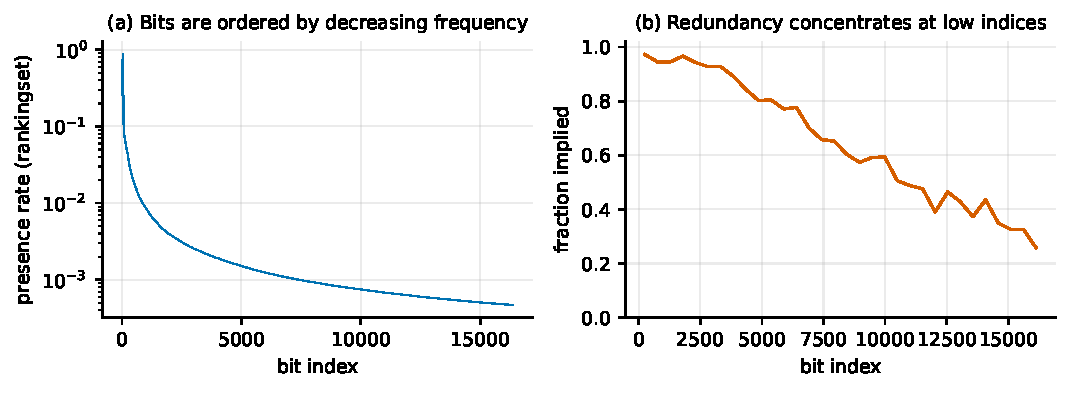
\includegraphics[width=\textwidth]{figs/fig1_ordering.pdf}
\caption{\textbf{The bit axis.} (a) Presence rate over the 518{,}901-molecule rankingset falls
monotonically with bit index, confirming that the entropy criterion is a frequency criterion.
(b) The fraction of bits that are logically implied by some other bit falls from $\approx$96\% at
low index to $\approx$32\% at high index --- the reason every index-dependent claim below is
reported within redundancy strata.}
\label{fig:ordering}
\end{figure}

\section{Result 1: mass bias is flat, not progressive}

For each of 16 equal bins define the mass ratio $\sum_j q_j / \sum_j p_j$, bootstrapped over
molecules ($B=2000$). If the model hedged on rare bits this ratio would decay with index. It does
not (Figure~\ref{fig:mass}, Table~\ref{tab:main}): there is a one-time step from 0.995 over the
first 1024 bits to $\approx$0.97, after which the ratio is flat to bit 16{,}383 --- the final bin
(0.9760) sits \emph{above} eight of the middle bins. Per molecule the shortfall is 57.5 predicted
mass against 58.3 true bits.

\begin{figure}[htbp]
\centering
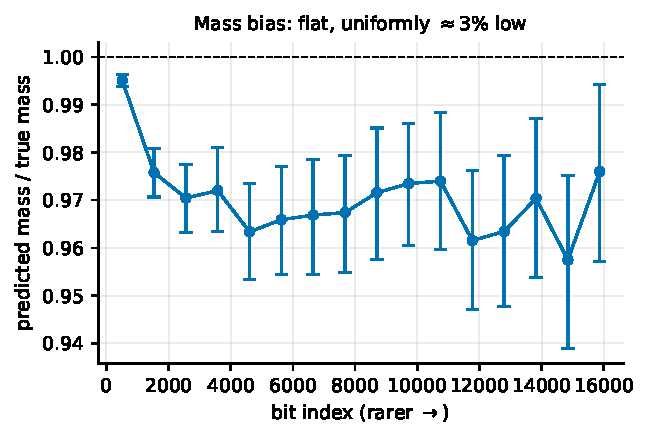
\includegraphics[width=0.52\textwidth]{figs/fig2_massbias.pdf}
\caption{\textbf{Predicted mass over true mass by bit index}, with 95\% bootstrap CIs over
molecules. A uniform $\approx$3\% deficit, not a decay. Widening CIs at high index reflect
positive counts thinning out, not increasing bias.}
\label{fig:mass}
\end{figure}

A per-bit Spearman correlation between relative bias $(q_j - p_j)/p_j$ and index is weakly negative
and significant ($\rho = -0.125$, $p = 8.7\times10^{-19}$, over the 5007 bits with $\geq$5
positives). This is worth stating precisely rather than either suppressing or over-reading: the
\emph{median} per-bit bias is $-0.0006$ while the \emph{mean} is $-0.031$. The bulk of late bits
are unbiased and the correlation is carried by a minority tail of badly-missed bits, which is a
different phenomenon from a shift of the distribution.

\section{Result 2: precision is flat, recall carries everything}

\begin{table}[htbp]
\centering
\small
\caption{Per-bin calibration and micro-averaged classification at threshold 0.5. \textbf{Precision
varies by 1.2 points across bins 2--16 while recall varies by 2.1 and drives every F1 movement.}
AUC is the mean over bits of the within-bit across-molecule ranking AUC.}
\label{tab:main}
\setlength{\tabcolsep}{4.6pt}
\begin{tabular}{lrrcrrrrrr}
\toprule
bit range & true rate & $q/p$ & 95\% CI & prec. & recall & F1 & FN & FP & AUC \\
\midrule
0--1023 & 0.03849 & 0.9951 & [0.9938, 0.9964] & 0.9819 & 0.9753 & 0.9786 & 2915 & 2129 & 0.9982 \\
1024--2047 & 0.00499 & 0.9758 & [0.9707, 0.9808] & 0.9651 & 0.9360 & 0.9503 & 980 & 518 & 0.9975 \\
2048--3071 & 0.00268 & 0.9705 & [0.9632, 0.9775] & 0.9664 & 0.9347 & 0.9503 & 538 & 268 & 0.9976 \\
3072--4095 & 0.00191 & 0.9720 & [0.9634, 0.9811] & 0.9595 & 0.9282 & 0.9436 & 422 & 230 & 0.9967 \\
4096--5119 & 0.00145 & 0.9633 & [0.9533, 0.9734] & 0.9614 & 0.9215 & 0.9410 & 350 & 165 & 0.9946 \\
5120--6143 & 0.00120 & 0.9659 & [0.9544, 0.9770] & 0.9615 & 0.9243 & 0.9425 & 278 & 136 & 0.9956 \\
6144--7167 & 0.00101 & 0.9669 & [0.9544, 0.9786] & 0.9594 & 0.9214 & 0.9400 & 244 & 121 & 0.9962 \\
7168--8191 & 0.00081 & 0.9674 & [0.9549, 0.9793] & 0.9653 & 0.9299 & 0.9472 & 174 & 83 & 0.9950 \\
8192--9215 & 0.00072 & 0.9716 & [0.9575, 0.9851] & 0.9548 & 0.9214 & 0.9378 & 175 & 97 & 0.9950 \\
9216--10239 & 0.00066 & 0.9735 & [0.9606, 0.9860] & 0.9615 & 0.9358 & 0.9485 & 130 & 76 & 0.9959 \\
10240--11263 & 0.00058 & 0.9740 & [0.9596, 0.9884] & 0.9549 & 0.9280 & 0.9412 & 128 & 78 & 0.9969 \\
11264--12287 & 0.00055 & 0.9615 & [0.9472, 0.9762] & 0.9592 & 0.9151 & 0.9367 & 144 & 66 & 0.9959 \\
12288--13311 & 0.00053 & 0.9634 & [0.9477, 0.9794] & 0.9574 & 0.9188 & 0.9377 & 131 & 66 & 0.9945 \\
13312--14335 & 0.00046 & 0.9704 & [0.9537, 0.9870] & 0.9613 & 0.9255 & 0.9431 & 106 & 53 & 0.9967 \\
14336--15359 & 0.00046 & 0.9575 & [0.9389, 0.9751] & 0.9589 & 0.9145 & 0.9362 & 122 & 56 & 0.9930 \\
15360--16383 & 0.00040 & 0.9760 & [0.9571, 0.9943] & 0.9570 & 0.9295 & 0.9430 & 86 & 51 & 0.9974 \\
\bottomrule
\end{tabular}
\end{table}

Micro-F1 steps from 0.9786 to $\approx$0.95 after the first 1024 bits and then holds between 0.9362
and 0.9503 across the remaining 15{,}360 bits, over which the base rate falls by a factor of 96.
The last bin (0.9430) beats four middle bins. Per-bit AUC is 0.993--0.998 with no trend. Macro
(per-bit) F1 is deliberately not reported: in the tail most bits have $\approx$1 positive across
3000 molecules, making per-bit F1 zero-or-one noise.

The decomposition is the informative part. \textbf{Precision is essentially constant} at
0.955--0.966 across bins 2--16, so the entire index dependence of F1 is a recall effect
(Figure~\ref{fig:prf}a). Precision exceeds recall in every single bin, equivalently FN $>$ FP in
every bin (Figure~\ref{fig:reliab}b) --- the same $\approx$3\% under-prediction seen in the mass
ratio, now visible as an error asymmetry. The model would rather miss a substructure than
hallucinate one, which for downstream retrieval is the benign direction.

\begin{figure}[htbp]
\centering
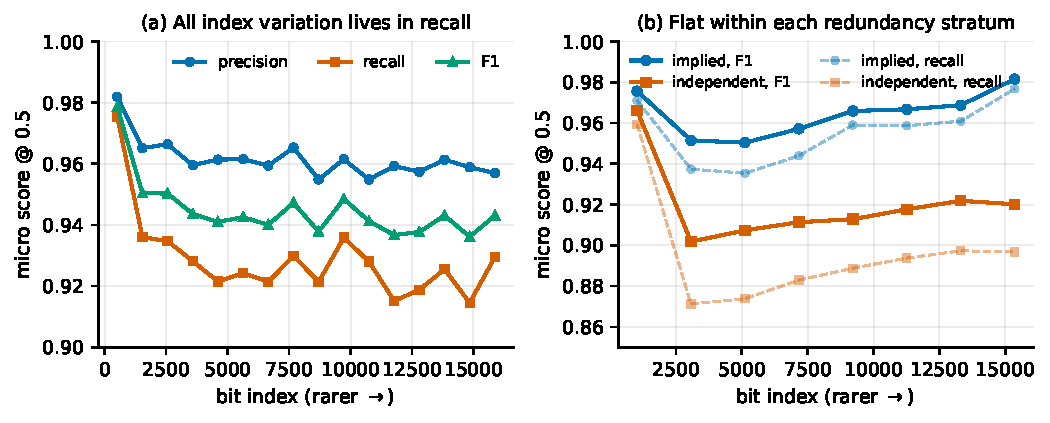
\includegraphics[width=\textwidth]{figs/fig3_prf.pdf}
\caption{\textbf{Micro precision / recall / F1 at threshold 0.5.} (a) Precision is flat by index;
recall carries all the variation, and the gap between them is the under-prediction. (b) Split by
redundancy stratum: both implied and independent bits are flat-to-rising toward rarer bits, and the
$\approx$6-point gap between strata is itself a recall gap, stable at every index.}
\label{fig:prf}
\end{figure}

\section{Result 3: the flatness survives the redundancy control}

Because implied bits fall from 96\% to 32\% of each octile, and implied bits score higher, an
unstratified curve could hide a genuine decay. It does not (Table~\ref{tab:strat}): within each
stratum the trend across the tail is flat or mildly \emph{increasing} --- independent bits go
0.9018 $\rightarrow$ 0.9201 in F1 from octile 2 to octile 8, implied bits 0.9515 $\rightarrow$
0.9815. The persistent $\approx$6-point gap between strata is a recall gap (precision differs by
$\approx$4 points, recall by $\approx$8), i.e.\ independent bits are \emph{missed} more often
rather than false-alarmed more often.

\begin{table}[htbp]
\centering
\small
\caption{Micro P/R/F1 at 0.5, stratified by whether a bit is logically implied by another bit.
Both strata are separately flat-to-rising with index, so the flat aggregate is not an artifact of
redundant bits propping up the tail.}
\label{tab:strat}
\begin{tabular}{lrrrrrrrr}
\toprule
& & \multicolumn{3}{c}{implied} & \multicolumn{3}{c}{independent} & \\
\cmidrule(lr){3-5}\cmidrule(lr){6-8}
bit range & \% impl. & prec. & recall & F1 & prec. & recall & F1 & $n_{+}$ (indep.) \\
\midrule
0--2047 & 95.8\% & 0.9802 & 0.9711 & 0.9756 & 0.9730 & 0.9593 & 0.9661 & 3075 \\
2048--4095 & 92.3\% & 0.9660 & 0.9374 & 0.9515 & 0.9346 & 0.8712 & 0.9018 & 1149 \\
4096--6143 & 80.6\% & 0.9658 & 0.9353 & 0.9503 & 0.9435 & 0.8738 & 0.9073 & 1664 \\
6144--8191 & 69.7\% & 0.9708 & 0.9439 & 0.9571 & 0.9416 & 0.8829 & 0.9113 & 1717 \\
8192--10239 & 59.1\% & 0.9728 & 0.9590 & 0.9659 & 0.9382 & 0.8888 & 0.9128 & 1861 \\
10240--12287 & 46.5\% & 0.9749 & 0.9586 & 0.9667 & 0.9429 & 0.8937 & 0.9176 & 1976 \\
12288--14335 & 42.5\% & 0.9767 & 0.9609 & 0.9687 & 0.9478 & 0.8973 & 0.9218 & 1860 \\
14336--16383 & 31.5\% & 0.9864 & 0.9767 & 0.9815 & 0.9447 & 0.8967 & 0.9201 & 1830 \\
\bottomrule
\end{tabular}
\end{table}

\paragraph{What ``implied'' means chemically.} The implication runs \emph{specific}
$\rightarrow$ \emph{general}, which is the opposite of what the name suggests. Over a 300-bit
sample of implied bits, the guaranteeing bit $j$ is a \emph{later, rarer} bit 83.7\% of the time
(median rankingset count 427 versus 595 for the bit it implies) and a \emph{larger-radius} fragment
66.7\% of the time. This is ECFP radius nesting: a large substructure contains the small core
inside it, so the small core is forced on whenever the large one fires (Table~\ref{tab:impl}).
An implied bit is therefore easy not because a common bit gives it away, but because it is a coarse
feature with many possible witnesses --- detecting \emph{any} enclosing fragment forces it. Pairs
with identical counts are the 1{,}695 two-way cases, where containment is mutual and the columns are
exact duplicates.

\begin{table}[htbp]
\centering
\footnotesize
\caption{Sampled implied bits and the bit that guarantees them ($r$ = ECFP radius, $c$ = rankingset
count). The antecedent is typically the rarer, larger fragment that structurally contains the
consequent.}
\label{tab:impl}
\resizebox{\textwidth}{!}{%
\begin{tabular}{rlrrrlrr}
\toprule
bit $i$ & fragment $i$ (implied) & $r_i$ & $c_i$ & bit $j$ & fragment $j$ (antecedent) & $r_j$ & $c_j$ \\
\midrule
4608 & \texttt{CC(C)NC(N)=O} & 2 & 854 & 9964 & \texttt{CCC1NC(=O)N(C)C1=O} & 3 & 390 \\
6983 & \texttt{CCC(OC)(OC)C(=O)O} & 2 & 551 & 7385 & \texttt{COC1(C(=O)O)CCC(N)C(C(C)O)O1} & 3 & 520 \\
10249 & \texttt{CCC(C(C)(C)C)C(C)(C)O} & 2 & 379 & 10392 & \texttt{CCC1C(C)(O)CC=C2CCCCC21C} & 3 & 374 \\
10937 & \texttt{CNc1ccc(C)cc1} & 3 & 355 & 12108 & \texttt{CNc1ccc(C(OC)C(C)N)cc1} & 4 & 322 \\
11081 & \texttt{cc(C)c1cc2c(C)coc2cc1o} & 4 & 351 & 11085 & \texttt{Cc1coc2cc3oc(=O)cc(C)c3cc12} & 4 & 351 \\
11719 & \texttt{CNC(=O)C(O)C(C)(C)COP(=O)(O)OP(=O)(O)O} & 5 & 333 & 11701 & \texttt{CC(C)(COP(=O)(O)OP)C(O)C(N)=O} & 4 & 333 \\
\bottomrule
\end{tabular}}
\end{table}

\section{Result 4: over-confidence is index-independent}

Whether rare bits are miscalibrated \emph{as probabilities} is a separate question from whether
they are ranked or thresholded well. Binning predictions by confidence and measuring the empirical
rate (Table~\ref{tab:reliab}, Figure~\ref{fig:reliab}a) gives four essentially superimposable
curves. The model is over-confident by the same margin everywhere: predictions near 0.964 are
correct 87\%, 88\%, 85\%, 85\% of the time for common, mid, rarest, and rarest-independent bits
respectively. There is no rare-bit-specific miscalibration to correct.

The one quantity that does move is the miss rate: 2.5\% of positives fall below 0.5 for the common
bits, 6.9\% mid, 7.6\% rarest, and 10.6\% for rarest-and-independent --- again a recall effect, and
again a step rather than a slope.

\begin{table}[htbp]
\centering
\small
\caption{Reliability by confidence bucket. Rows are near-identical across bit groups; the model's
over-confidence does not depend on bit rarity.}
\label{tab:reliab}
\begin{tabular}{lrrrrrr}
\toprule
& \multicolumn{2}{c}{0--1023 (common)} & \multicolumn{2}{c}{8192--16383 (rarest)} & \multicolumn{2}{c}{8192--16383 indep.} \\
\cmidrule(lr){2-3}\cmidrule(lr){4-5}\cmidrule(lr){6-7}
confidence & $n$ & empirical & $n$ & empirical & $n$ & empirical \\
\midrule
$[0.5, 0.7)$    & 1081 & 0.5273 & 302 & 0.5397 & 237 & 0.5316 \\
$[0.7, 0.9)$    & 1783 & 0.6826 & 508 & 0.6831 & 380 & 0.7263 \\
$[0.9, 0.99)$   & 4543 & 0.8734 & 1096 & 0.8522 & 844 & 0.8531 \\
$[0.99, 0.999)$ & 8060 & 0.9695 & 1602 & 0.9713 & 1129 & 0.9681 \\
$[0.999, 1)$    & 101977 & 0.9977 & 9423 & 0.9963 & 4544 & 0.9936 \\
\midrule
missed positives & \multicolumn{2}{c}{0.0247} & \multicolumn{2}{c}{0.0762} & \multicolumn{2}{c}{0.1059} \\
\bottomrule
\end{tabular}
\end{table}

\begin{figure}[htbp]
\centering
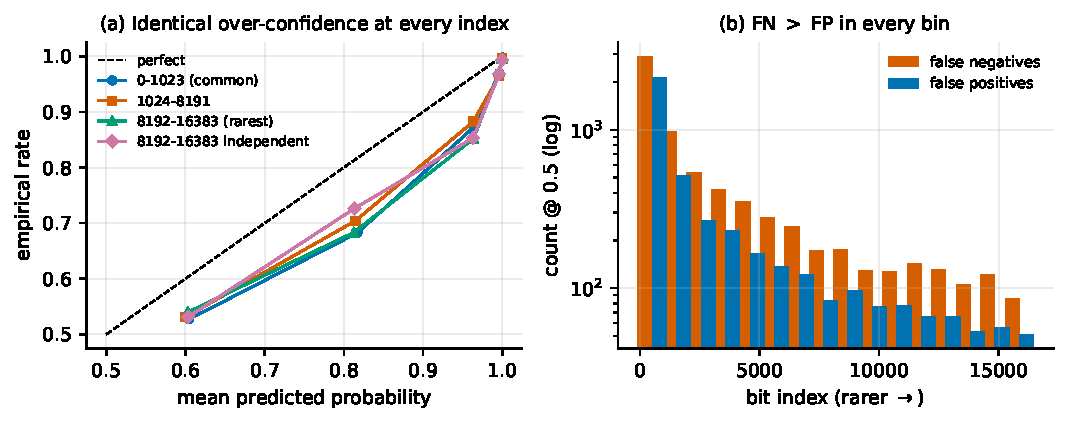
\includegraphics[width=\textwidth]{figs/fig4_reliability.pdf}
\caption{(a) \textbf{Reliability diagrams} for four bit groups spanning the full rarity range; the
curves lie on top of each other, all below the diagonal by the same margin. (b) \textbf{False
negatives exceed false positives in every bin} (log scale), the error-side view of the uniform
$\approx$3\% mass deficit.}
\label{fig:reliab}
\end{figure}

\begin{figure}[htbp]
\centering
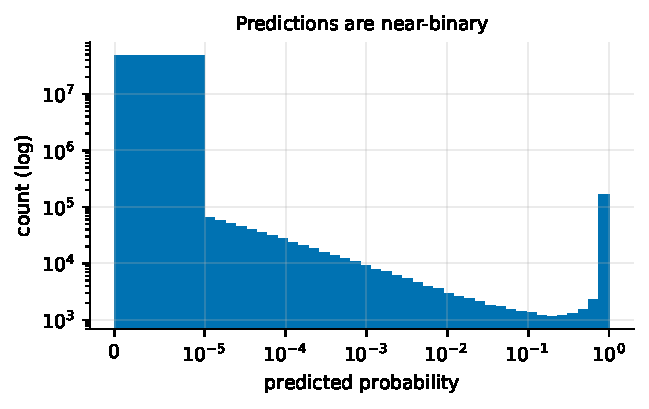
\includegraphics[width=0.52\textwidth]{figs/fig5_sharpness.pdf}
\caption{\textbf{Predictions are near-binary.} 99.26\% of the 49.2M predicted probabilities fall
below $10^{-4}$ and 0.34\% exceed 0.9, leaving $<$0.06\% in the middle. The head is decisive rather
than hedging --- consistent with a model that is not shrinking rare-bit outputs toward the base
rate.}
\label{fig:sharpness}
\end{figure}

\section{Caveats}

\begin{enumerate}\itemsep0.2em
\item \textbf{Tail sample size.} 3000 test molecules means the final bin rests on 1{,}220 positives
and only 42 of its 2048 bits have $\geq$5 positives. The $\pm$0.01 wobble between adjacent late
bins is not interpretable; the flatness claim rests on the absence of a trend across sixteen bins,
not on any single bin. Re-running \texttt{01\_predict.py --limit 0} over the full test split would
tighten this.
\item \textbf{Threshold choice.} P/R/F1 are reported at 0.5. Given the near-binary output
distribution (Figure~\ref{fig:sharpness}) the numbers are insensitive to this within a wide range,
but they are not threshold-free; AUC and the mass ratio are, and they agree.
\item \textbf{Single checkpoint, single split.} All results are \texttt{final1} on the MARINA1 test
split. Nothing here is seed-averaged.
\item \textbf{The Spearman trend is real but small.} Reported in Section 2 rather than dismissed:
$\rho = -0.125$ is statistically solid and directionally consistent with mild extra
under-prediction of rare bits. The claim being defended is that its magnitude (median bias
$-0.0006$) is negligible relative to the 96$\times$ change in base rate, not that it is zero.
\end{enumerate}

\section{Conclusion}

MARINA is learning the rare tail of the fingerprint appropriately. There is a genuine
under-prediction bias --- about 3\% of mass, visible as FN $>$ FP in every bin and as
precision-above-recall throughout --- but it is uniform in bit index rather than concentrated in
the rare bits. Across the 15{,}360 bits after the first 1024, base rate falls 96$\times$ while F1
stays within 0.936--0.950, AUC within 0.993--0.998, and reliability curves remain superimposable.
The single index-dependent effect in the entire analysis is recall, and it is a one-time step at
bit $\approx$1024, not a decay. Stratifying by logical implication --- necessary because redundant
bits are 3$\times$ over-represented at low indices --- leaves both strata separately flat.

The practical implications: (i) there is no case for a rarity-dependent loss reweighting or
per-bit threshold calibration, since neither the bias nor the over-confidence depends on index;
(ii) the uniform under-prediction is in the safe direction for retrieval and could be removed
globally with a single threshold shift if desired; (iii) the wasted capacity documented in the
companion MI-redundancy analysis is a \emph{selection} problem, not a \emph{learning} problem ---
the model extracts what is there, so any gain must come from choosing better bits rather than from
fitting the current ones harder.

\vspace{1em}
\hrule
\vspace{0.5em}
{\footnotesize
\textbf{Reproduce:}
\texttt{cd Datasets/fp-redundancy \&\& pixi run python scripts/10\_bit\_calibration.py} (tables),
\texttt{scripts/11\_report\_figures.py} (figures + \texttt{report/stats.json}).
Both consume \texttt{results/preds.npz} and \texttt{results/bit\_mi.npz}.
Compile: \texttt{tectonic report/bit-calibration.tex}.
}

\end{document}
